\documentclass{tufte-handout}
\usepackage{graphicx}
\graphicspath{ {./images/} }
\renewcommand{\vec}[1]{\mathbf{#1}} %make \vec command turn vectors bold instead

\author{Andr\'es Ponce}
\title{Ensemble Methods}

\begin{document}
\maketitle
\begin{abstract}
	\textbf{Ensemble Methods} refer to when we use an aggregate of $L$ different
	models to find more accurate predictions for our data. There are several 
	ways of implementing a selection from several methods: adaboost, decision trees,
	bagging, random forests, etc...	
\end{abstract}

\section{Boosting}
The straightforward approach to using multiple models is to take the average value of each of the 
models that we use. Supposing we want to use $M$ models, and we want to predict the value given 
by a certain function, we could say 
\[y_{COM} = \frac{1}{M} \sum_{m = 1}^{M}y_{m}(x)\]

where $COM$ refers to the \textit{decision by committee} given by the equations. We take the average
value of the $M$ models to form our final result. When calculating the error, we also take the aggregate
error of all the models.

\textbf{Boosting} then refers to the building of a strong classifier for a problem by using several weaker
classifiers. When boosting, we again can have $M$ models whose scores are summed up. 

\begin{marginfigure}
	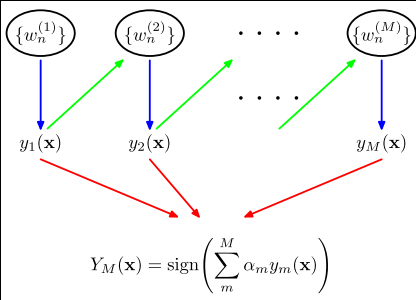
\includegraphics[scale=0.4]{adaptive}
	\caption{Each of the models contributes to how we pass the input set to the next model to be trained. 
	At the end, we also use each model's results to calculate the final prediction.}
\end{marginfigure}
The type of boosting called \textbf{Adaptive Boosting} will pass the input through the models
sequentially, and \textit{train} the models sequentially. Then, when training the next model, items that 
were misclassified will be given greater weight. This may result in an overall model which performs 
very well even if the models themselves perform as well as random ones.

The process for AdaBoost looks something like:
\begin{enumerate}
	\item Given inputs $(x_{1}, y{1}),...,(x_{m},y_{m})$ where $x_{i} \in X, y_{i} \in\{-1, +1\}$,
			initialize their distributions $D_{t}(i)= \frac{1}{m}, i = 1,...,m$
			\footnote{The distributions $D_{t}(i)$ mean the probability distribution of $x_{i}$'s at time $t$}
	\item Find the classifier $h_{t}$ which minimizes the error w.r.t. $D_{t}$.\footnote{We can basically take
			the min of 
				\[\epsilon_{j} = \sum_{i = 1}^{m}D_{t}(i)[y_{i} \neq h_{j}(x_{i})]\]}
	\item Calculate the weight classifier $\alpha_{t} = \frac{1}{2}ln\frac{1 - \epsilon_{t}}{\epsilon{t}}$
	\item Update our distribution \footnote{ $Z_{t}$ is basically a value to normalize the distribution.}
			\[ D_{t + 1}(i) = \frac{D_{t}\textrm{exp}[-\alpha_{t}y_{i}h_{t}(x_{i})]}{Z_{t}} \]
\end{enumerate}

Once we have the final classifier $H(x)$, comprised of the sum of the modesl with the adjusted weights and
distributions, we can calculate the \textbf{margin} of the classifier on a sample $(x, y)$. The margin is
given by \footnote{The margin tells us when we classified the input correctly, and our confidence with our 
classification.}
\[yH(x)\]

The AdaBoost algorithm will try to maximize the margins of our variables by minimizing the 
\textbf{exponential loss} of the predictions.
\[loss_{exp}[H(x)]= E_{x,y}[e^{-yH(x)}]\]

\end{document}
